\documentclass[11pt]{article}

% set these commands
\newcommand{\course}{CSCI 347}
\newcommand{\proj}{Homework 03}

\usepackage{macros}
\usepackage{tcolorbox}


\begin{document}

{ ~\\
    River Kelly \\
    \course \\ 
    \proj \\ 
}

Show your work. Include any code snippets you used to generate an answer, using
comments in the code to clearly indicate which problem corresponds to which code

Consider the following graph:

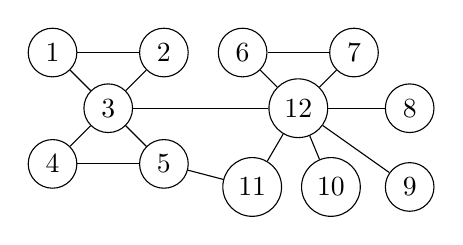
\begin{tikzpicture}[main/.style = {draw, circle}]

\node[main] (3) {3};
\node[main] (1) [above left of=3] {1};
\node[main] (2) [above right of=3] {2};
\node[main] (4) [below left of=3] {4};
\node[main] (5) [below right of=3] {5};


\node[main] (6) [right of=2] {6};
\node[main] (12) [below right of=6] {12};
\node[main] (7) [above right of=12] {7};
\node[main] (8) [below right of=7] {8};
\node[main] (9) [below of=8] {9};
\node[main] (10) [left of=9] {10};
\node[main] (11) [left of=10] {11};

\draw[-] (1) -- (2);
\draw[-] (1) -- (3);
\draw[-] (2) -- (3);

\draw[-] (3) -- (4);
\draw[-] (3) -- (5);
\draw[-] (3) -- (12);

\draw[-] (4) -- (5);
\draw[-] (5) -- (11);

\draw[-] (6) -- (7);
\draw[-] (6) -- (12);
\draw[-] (7) -- (12);
\draw[-] (8) -- (12);
\draw[-] (9) -- (12);
\draw[-] (10) -- (12);
\draw[-] (11) -- (12);

\end{tikzpicture}

Answer the following:

\begin{enumerate}

    \item (3 points) Without using networkx or other graph analysis packages
    (though you may use them to check your answer), find the closeness
    centrality of vertices 3 and 12.
    \begin{align*}
        cc(x_{3}) &= \frac{1}{\sum_{j=1}^{n} d( x_3 , x_j )} \\
        &= \frac{1}{1 + 1 + 0 + 1 + 1 + 2 + 2 + 2 + 2 + 2 + 2 + 1} \\
        &= \frac{1}{17} \\
        &= 0.05882352....
    \end{align*}
    \begin{align*}
        cc(x_{12}) &= \frac{1}{\sum_{j=1}^{n} d( x_{12} , x_j )} \\
        &= \frac{1}{2+2+1+2+2+1+1+1+1+1+1+0} \\
        &= \frac{1}{15} \\
        &= 0.06666666....
    \end{align*}
    \begin{tcolorbox}[width=\linewidth,title=Problem 1 Answer - Closeness Centrality]
        The closeness centrality of vertex 3: $\frac{1}{17}$ or $0.059$ \\
        The closeness centrality of vertex 12: $\frac{1}{15}$ or $0.067$
    \end{tcolorbox}

    \newpage
    \item (3 points) Without using networkx or other graph analysis packages
    (though you may use them to check your answer), find the eccentricity of
    vertices 3, 12, and 11.
    \begin{align*}
        e(x_i) &= \max_{i} \lbrace d( x_{i} , x_{j} ) \rbrace \\
        e(x_3) &= 2 \\
        e(x_{12}) &= 2 \\
        e(x_{11}) &= 3
    \end{align*}
    \begin{tcolorbox}[width=\linewidth,title=Problem 2 Answer - Eccentricity]
        The eccentricity of vertex 3: $2$ \\
        The eccentricity of vertex 12: $2$ \\
        The eccentricity of vertex 11: $3$
    \end{tcolorbox}

    \item (3 points) Without using networkx or other graph analysis packages
    (though you may use them to check your answer), find the clustering
    coefficient of vertex 3.
    \begin{align*}
        \frac{ m_{i} }{ ( \substack{ n_{i} \\ 2} ) } &= \frac{ \text{\# of edges amoung neighbors of } x_{i} }{ \text{\# of possible edges amoung neighbors of } x_{i} } \\
        \frac{ m_{3} }{ ( \substack{ n_{3} \\ 2} ) } &= \frac{2}{10} \\
        &= \frac{1}{5}
    \end{align*}

    \item (3 points) Without using networkx or other graph analysis packages
    (though you may use them to check your answer), find the clustering
    coefficient of the graph.

    \item (3 points) Find the betweenness centrality of vertices 3 and 12. You
    may use networkx or other graph analysis packages, but include the code used
    to generate your answer in your submission.

    \item (3 points) Using networkx, find the prestige centrality of vertices 3
    and 12. Include the code used to generate the answer. (Note that networkx
    calls the prestige centrality ``eigenvector centrality'')

    \item (3 points) Use Python to create a plot for the degree distribution of
    this graph.  Include the code used to generate the plot as well as the plot
    in your submission.

\end{enumerate}

{\bf Acknowledgements:} Homework problems adapted from assignments of
Veronika Strnadova-Neeley.

\end{document}
